%Listing definition for XML

\definecolor{gray}{rgb}{0.4,0.4,0.4}
\definecolor{darkblue}{rgb}{0.0,0.0,0.6}
\definecolor{cyan}{rgb}{0.0,0.6,0.6}

\lstset{
  basicstyle=\ttfamily,
  columns=fullflexible,
  showstringspaces=false,
  commentstyle=\color{gray}\upshape
}

\lstdefinelanguage{XML}
{
  morestring=[b]",
  morestring=[s]{>}{<},
  morecomment=[s]{<?}{?>},
  stringstyle=\color{black},
  identifierstyle=\color{darkblue},
  keywordstyle=\color{cyan},
  morekeywords={}% list your attributes here
}

%%%%%%%%%%%%%%%%%%%%%%%%%%%%%%%%%%%%%%%%%%%%%%%%%%%%%%%%%%%%%%%%%%%%%%%%%%%%%

%Listing definition for Java
\definecolor{javared}{rgb}{0.6,0,0} % for strings
\definecolor{javagreen}{rgb}{0.25,0.5,0.35} % comments
\definecolor{javapurple}{rgb}{0.5,0,0.35} % keywords
\definecolor{javadocblue}{rgb}{0.25,0.35,0.75} % javadoc

\lstset{prebreak=\raisebox{0ex}[0ex][0ex]
        {\ensuremath{\rhookswarrow}}}
\lstset{postbreak=\raisebox{0ex}[0ex][0ex]
        {\ensuremath{\rcurvearrowse\space}}}
\lstset{breaklines=true, breakatwhitespace=true}
\lstset{numbers=left, numberstyle=\scriptsize}
 
\lstset{language=Java,
basicstyle=\ttfamily,
keywordstyle=\color{javapurple}\bfseries,
stringstyle=\color{javared},
commentstyle=\color{javagreen},
morecomment=[s][\color{javadocblue}]{/**}{*/},
numbers=left,
numberstyle=\tiny\color{black},
stepnumber=2,
numbersep=10pt,
tabsize=4,
showspaces=false,
showstringspaces=false
}

%%%%%%%%%%%%%%%%%%%%%%%%%%%%%%%%%%%%%%%%%%%%%%%%%%%%%%%%%%%%%%%%%%%%%%%%%%%%%%%%%

\chapter{Implementation}

\section{Technologies used}

As it has been explained previously, the two modules developed as part of the work for this thesis have been designed to be integrated with the Hummingbird project. To do so, Java\cite{Java} has been chosen as the main programming language, as it is the language used for the development of Hummingbird. In the same way, Apache Camel\cite{Camel} and ActiveMQ \cite{AMQ} are used for the communication with the rest of the modules. XStream\cite{XStream} has been chosen as the library used to parse the XML files used to specify the scientific information.

The final piece of technology used is BeanShell\citep{BSH}, a Java-like scripting language and interpreter which runs in the Java Runtime Environment. The calibration module has been designed to be generic, adaptable to every mission. Also, the goal was to make the calibration information input easy for the scientists, meaning this no need to any difficult Java programming, compilation and so on. BeanShell integrates with the Java code and allows to run those scripts \textbf{in (under, on????)} runtime.

\section{Implementation of the calibration module}

For the sake of clarity, the approach to the explanation will be in small pieces. However, before jumping onto every small piece, it is interesting to look at the package organization of the module.

The software is divided into several Java packages being those the following:
\begin{itemize}
\item \textbf{eu.estcube.calibration}: provided by the \emph{Hummingbird} software architect, it contains the Apache Camel integration. It also contains the main class of the module.
\item \textbf{eu.estcube.calibration.calibrate}: contains the implementation of the calibrator.
\item \textbf{eu.estcube.calibration.constants}: contains several constants used throughout the module.
\item \textbf{eu.estcube.calibration.domain}: contains the data structures used to represent the calibration information and the calibration units.
\item \textbf{eu.estcube.calibration.processors}: contains the main algorithm for receiving, calibrating and sending the parameters back. Also, the interface implemented by the calibrator can be found here.
\item \textbf{eu.estcube.calibration.utils}: contains additional utilities. In this case, the tools to manage finding and reading files.
\item \textbf{eu.estcube.calibration.xmlparser}: contains the tools to parse the information contained in XML format into data which can be used in the module.
\end{itemize}

\subsection{Camel Integration}

The integration with Camel is a crucial part of the module since it is where it will take the parameters from. There are several classes related to this, the class diagram of this part can be seen in Figure \ref{f5.1}. 

\begin{figure}[H]
\centerline{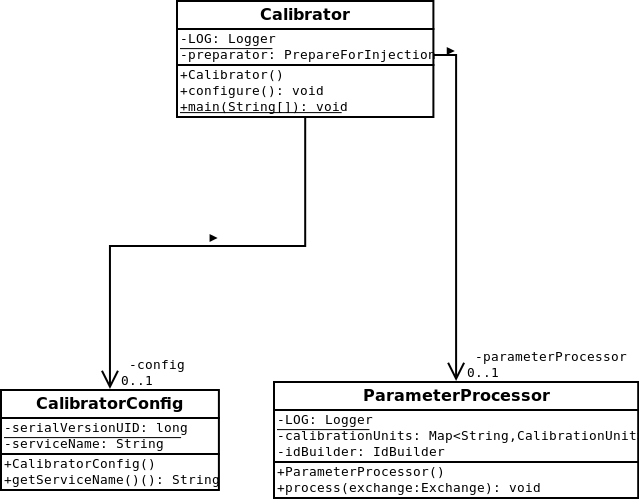
\includegraphics[width=0.75\textwidth]{images/CalibratorCamelClassDiagram.png}}
\caption{Class diagram of the Camel integration}
\label{f5.1}
\end{figure}

Amongst the three classes represented in Figure \ref{f5.1} it is important to highlight two of them: \emph{Calibrator} and \emph{ParameterProcessor}.

\emph{Calibrator} is the main class of the module. As it is shown in the class diagram there are two methods, the \textbf{main} method, where everything starts and the \textbf{configure} method. The latter is where the integration with Camel happens, what configures where to get the messages from, what to do with them and where to send them afterwards. In addition, \emph{Hummingbird} utilizes a heartbeat system to check if the modules are working correctly, this is also carried on here. To see a snippet of the code see Table \ref{Table5.1}.

\begin{table}[h]
\lstset{language=Java}
\begin{lstlisting}

    @Override
    public void configure() throws Exception {

        // @formatter:off
        from(StandardEndpoints.MONITORING)
            .filter(header(StandardArguments.CLASS)
            .isEqualTo(Parameter.class.getSimpleName()))
            .process(parameterProcessor)
            .split(body())
            .process(preparator)
            .to(StandardEndpoints.MONITORING);
        
        BusinessCard card = new BusinessCard(config.getServiceId(), config.getServiceName());
        card.setPeriod(config.getHeartBeatInterval());
        card.setDescription(String.format("Calibrator; version: %s", config.getServiceVersion()));
        from("timer://heartbeat?fixedRate=true&period=" + config.getHeartBeatInterval())
            .bean(card, "touch")
            .process(preparator)
            .to(StandardEndpoints.MONITORING);
        // @formatter:on

    }



\end{lstlisting}
\caption{Camel integration Java code}
\label{Table5.1}
\end{table}

\pagebreak
Focusing on the part where the module receives and sends the parameters we can see that:

\begin{itemize}
\item Where it gets the messages from --> \emph{from(StandardEndpoints.MONITORING)}
\item It only gets messages containing parameters -->  \emph{.filter(header(StandardArguments.CLASS)}
            \emph{.isEqualTo(Parameter.class.getSimpleName()))}
\item What to do with the received message --> \emph{.process(parameterProcessor)}
\item Since the result of the processed message is a list and it is necessary to send the parameters one by one, that result must be split. --> \emph{.split(body())}
\item Send it back to the messaging service --> \emph{.process(preparator)}\linebreak
            \emph{.to(StandardEndpoints.MONITORING);}

\end{itemize}


The second part - from line 14 and below - contains the heartbeat system.


\emph{ParameterProcessor} contains the following:
\begin{itemize}
\item Part of the Camel integration.
\item Code to load the calibration information from the configuration files.
\item Algorithm to process the received parameters.
\end{itemize}




For each entry in the XML file, one instance of the above data structure is created and then stored in a \textbf{HashMap}. The reason for choosing this data structure is its efficiency. It provides constant-time performance for the input and retrieval of information\cite{HashMap}.


Figure xx represents the sequence diagram of this part of the software.

\begin{figure}[H]
\centerline{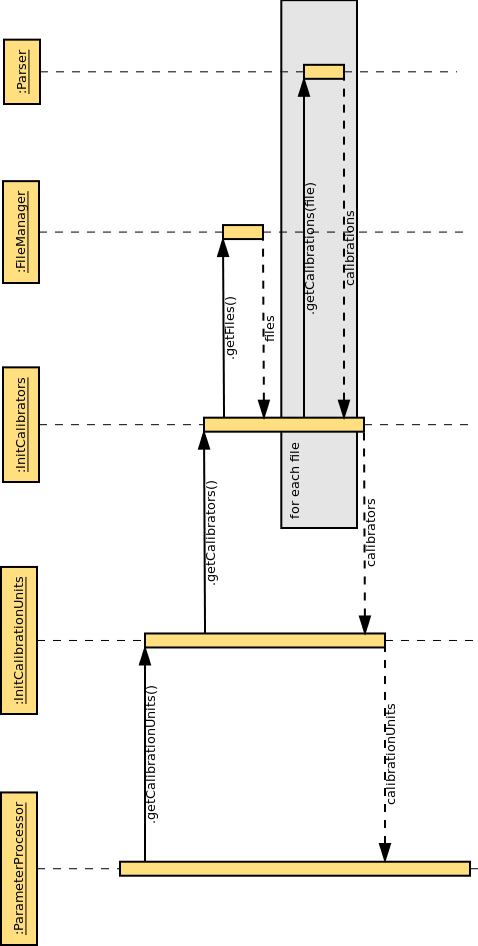
\includegraphics[width=0.75\textwidth]{images/InitCalibrationUnitsSequence.png}}
\caption{Semimajor Axis}
\label{f2.1}
\end{figure}









\section{Implementation of the limit checking module}


\section{User manual}
\subsection{Calibration module}
This short user manual covers the use of the calibration module. The process is fully automated, so the user only needs to configure the pertinent XML file containing the information related to all the parameters which need to be calibrated.

There can be as many files as needed, although it is recommended to have one file per subsystem. This way, the person who is making the changes will not have to be worried about modifying some other parts they do not understand. It is advisable that each file is called as the corresponding subsystem.


The location of the folder where the XML files are stored is fully configurable by a system property. It can be set like this: \textbf{-Dpath="/path/to/the/folder"}.

The XML file has the following format:
\begin{table}[h]
\lstset{language=XML}
\begin{lstlisting}

<calibration>
	<entry>
		<id></id>
		<description></description>
		<outputId></outputId>
		<unit></unit>
		<scriptInfo>
			<isVector></isVector>
			<resultVariable></resultVariable>
			<auxParameters></auxParameters>
			<script></script>
		</scriptInfo>
	</entry>
</calibration>
\end{lstlisting}
\caption{blablabla}
\label{Table5.890}
\end{table}

\begin{itemize}
\item \textbf{id}: name of the parameter to calibrate.
\item \textbf{Description}: description of the parameter.
\item \textbf{outputId}: name of the parameter generated after the calibration. If left blank, it will be the same as \textbf{id}. Please note that all calibrated parameters names end in \textbf{\_cal}.
\item \textbf{unit}: Units in which the value is represented.
\item \textbf{isVector}: \textbf{true} if the result of the calibration is a vector with several values (which generates several new parameters) or \textbf{false} if the calibration returns a single value.
\item \textbf{resultVariable}: variable in the script in which the result will be stored.
\item \textbf{auxParameters}: if the are extra parameters needed for the calibration process it is necessary to list them here separated by commas (','). Please note that if the extra parameters also needs to be calibrated the parameters needed for its calibration also must be included here insted of the original one (See Figure \ref{f23}).
\item \textbf{script}: script to generate the calibrated value. Please note that if extra parameters are needed, their calibration script must be included here, not the parameter name (See Figure \ref{}). 
\end{itemize}



\begin{table}[H]
\lstset{language=XML}
\begin{lstlisting}

<calibration>
	<entry>
		<id>parameterA</id>
		<description>Example of parameter for
		 simple calibration</description>
		<outputId>generatedA</outputId> 
		<unit>E</unit>
		<scriptInfo>
			<isVector>false</isVector>
			<resultVariable>result</resultVariable>
			<auxParameters></auxParameters>
			<script>result = (parameterA*779.09823)/3145.2839</script>
		</scriptInfo>
	</entry>
</calibration>
\end{lstlisting}
\caption{Example of simple calibration}
\label{Table5.2}
\end{table}

Figure \ref{f5.4} represents the simplest example of calibration information. \textbf{parameterA} is the parameter to be calibrated and the user has chosen that the name of the calibrated parameter will be \textbf{generatedA}. The software will automatically append  \_cal, so the final output name will be \textbf{generatedA\_cal}. The information about the calibration script states that the result will not be a vector and the value after the calculations will be stored in a variable called \textbf{result}. There are no extra parameters needed ant the calibration script is $(parameterA*779.09823)/3145.2839$.

\begin{table}[H]
\lstset{language=XML}
\begin{lstlisting}

<calibration>
	<entry>
		<id>parameterA</id>
		<description>Example of parameter which depends
		 on others to be calibrated</description>
		<outputId></outputId>\section{Design}
		<unit>E</unit>
		<scriptInfo>
			<isVector>false</isVector>
			<resultVariable>result</resultVariable>
			<auxParameters>parameterB,parameterC</auxParameters>
			<script>result = (parameterA*(parameterB*2345/37))
			/3145.2839 + (parameterC*2)</script>
		</scriptInfo>
	</entry>
</calibration>
\end{lstlisting}
\caption{Example of calibration depending on other parameters}
\label{Table5.3}
\end{table}

Figure \ref{f5.4} shows an example of a parameter which depends on others for calibration. Again, \textbf{parameterA} is the name of the parameter to be calibrated. In this case the user has not selected an output ID, so it will by default be \textbf{parameterA\_cal}. The result of the calibration will not be a vector and it needs \textbf{parameterB} and \textbf{parameterC} to be calibrated. The calibration script can be explained as follows:
\begin{itemize}
\item Calibration script for \textbf{parameterA}: $result = ((parameterA*(parameterB\_cal))\\			/3145.2839) + (parameterC\_cal)$
\item Instead of just stating that \textbf{parameterB\_cal} is needed to carry on the calibration, the user must specify its calibration script: $parameterB*2345/37$
\item Same thing with \textbf{parameterC\_cal}: $parameterC*2$
\item The final result is what can be seen in the example: $result = (parameterA*(parameterB*2345/37))/3145.2839 + (parameterC*2)$
\end{itemize}
\begin{table}[H]
\lstset{language=XML}
\begin{lstlisting}

<calibration>
	<entry>
		<id>parameterA</id>
		<description>Example of parameter for simple calibration</description>
		<outputId>generatedA</outputId>
		<unit>E</unit>
		<scriptInfo>
			<isVector>false</isVector>
			<resultVariable>result</resultVariable>
			<auxParameters></auxParameters>
			<script>result = (parameterA*779.09823)/3145.2839</script>
		</scriptInfo>
	</entry>
</calibration>
\end{lstlisting}
\caption{Example of simple calibration}
\label{Table5.4}
\end{table}


\subsection{Limit checking module}
This subsection covers the user manual for the limit checking module. The process is fully automated, so the user only needs to configure the pertinent XML file containing the information related to the limits of every parameter. 

There can be as many files as needed, although it is recommended to have one file per subsystem. This way, the person who is making the changes will not have to be worried about modifying some other parts they do not understand.It is advisable that each file is called as the corresponding subsystem.

The location of the folder where the XML files are stored is fully configurable by a system property. It can be set like this: \textbf{-Dpath="/path/to/the/folder"}.

The XML file has the following format:
\begin{table}[H]
\lstset{language=XML}
\begin{lstlisting}

<limitChecking>
	<entry>
		<id></id>
		<limits>
			<sanityLower></sanityLower>
			<hardLower></hardLower>
			<softLower></softLower>
			<softUpper></softUpper>
			<hardUpper></hardUpper>
			<sanityUpper></sanityUpper>
		</limits>
	</entry>
</limitChecking>
\end{lstlisting}
\caption{blablabla}
\label{Table5.5}
\end{table}

\begin{itemize}
\item \textbf{id}: name of the parameter to calibrate which limits are to be checked.
\item \textbf{Sanity limits}: Optional. If the value is below the lower limit or above the upper limit it is discarded. 
\item \textbf{Hard limits}:
	\begin{itemize}
	\item If the sanity limits are available anything between these limits and the sanity limits is considered an error.
	\item If the sanity limits are disabled anything below the lower limit or above the upper limit is considered an error. 
	\end{itemize}
\item \textbf{Soft limits}: 
\begin{itemize}
\item Anything between the lower and upper soft limits is considered an OK value.
\item Anything between the soft limits and the hard limits is considered OK, but with a warning.
\end{itemize}
\end{itemize}

The following two examples show the two ways in which the limit checking module can be configured:

\begin{table}[H]
\lstset{language=XML}
\begin{lstlisting}
<limitChecking>
	<entry>
		<id>parameterA</id>
		<limits>
			<sanityLower>-100</sanityLower>
			<hardLower>-75</hardLower>
			<softLower>-20</softLower>
			<softUpper>20</softUpper>
			<hardUpper>75</hardUpper>
			<sanityUpper>100</sanityUpper>
		</limits>
	</entry>
</limitChecking>
\end{lstlisting}
\caption{Limit checking with sanity limits available}
\label{Table5.6}
\end{table}

\begin{table}[H]
\lstset{language=XML}
\begin{lstlisting}
<limitChecking>
	<entry>
		<id>parameterA</id>
		<limits>
			<hardLower>-75</hardLower>
			<softLower>-20</softLower>
			<softUpper>20</softUpper>
			<hardUpper>75</hardUpper>
		</limits>
	</entry>
</limitChecking>
\end{lstlisting}
\caption{Limit checking without sanity limits available}
\label{Table5.7}
\end{table}


\newpage

